% Options for packages loaded elsewhere
\PassOptionsToPackage{unicode}{hyperref}
\PassOptionsToPackage{hyphens}{url}
%
\documentclass[
]{article}
\title{SRI Interview App (PDF)}
\author{Trubin Filipp}
\date{1/11/2022}

\usepackage{amsmath,amssymb}
\usepackage{lmodern}
\usepackage{iftex}
\ifPDFTeX
  \usepackage[T1]{fontenc}
  \usepackage[utf8]{inputenc}
  \usepackage{textcomp} % provide euro and other symbols
\else % if luatex or xetex
  \usepackage{unicode-math}
  \defaultfontfeatures{Scale=MatchLowercase}
  \defaultfontfeatures[\rmfamily]{Ligatures=TeX,Scale=1}
\fi
% Use upquote if available, for straight quotes in verbatim environments
\IfFileExists{upquote.sty}{\usepackage{upquote}}{}
\IfFileExists{microtype.sty}{% use microtype if available
  \usepackage[]{microtype}
  \UseMicrotypeSet[protrusion]{basicmath} % disable protrusion for tt fonts
}{}
\makeatletter
\@ifundefined{KOMAClassName}{% if non-KOMA class
  \IfFileExists{parskip.sty}{%
    \usepackage{parskip}
  }{% else
    \setlength{\parindent}{0pt}
    \setlength{\parskip}{6pt plus 2pt minus 1pt}}
}{% if KOMA class
  \KOMAoptions{parskip=half}}
\makeatother
\usepackage{xcolor}
\IfFileExists{xurl.sty}{\usepackage{xurl}}{} % add URL line breaks if available
\IfFileExists{bookmark.sty}{\usepackage{bookmark}}{\usepackage{hyperref}}
\hypersetup{
  pdftitle={SRI Interview App (PDF)},
  pdfauthor={Trubin Filipp},
  hidelinks,
  pdfcreator={LaTeX via pandoc}}
\urlstyle{same} % disable monospaced font for URLs
\usepackage[margin=1in]{geometry}
\usepackage{color}
\usepackage{fancyvrb}
\newcommand{\VerbBar}{|}
\newcommand{\VERB}{\Verb[commandchars=\\\{\}]}
\DefineVerbatimEnvironment{Highlighting}{Verbatim}{commandchars=\\\{\}}
% Add ',fontsize=\small' for more characters per line
\usepackage{framed}
\definecolor{shadecolor}{RGB}{248,248,248}
\newenvironment{Shaded}{\begin{snugshade}}{\end{snugshade}}
\newcommand{\AlertTok}[1]{\textcolor[rgb]{0.94,0.16,0.16}{#1}}
\newcommand{\AnnotationTok}[1]{\textcolor[rgb]{0.56,0.35,0.01}{\textbf{\textit{#1}}}}
\newcommand{\AttributeTok}[1]{\textcolor[rgb]{0.77,0.63,0.00}{#1}}
\newcommand{\BaseNTok}[1]{\textcolor[rgb]{0.00,0.00,0.81}{#1}}
\newcommand{\BuiltInTok}[1]{#1}
\newcommand{\CharTok}[1]{\textcolor[rgb]{0.31,0.60,0.02}{#1}}
\newcommand{\CommentTok}[1]{\textcolor[rgb]{0.56,0.35,0.01}{\textit{#1}}}
\newcommand{\CommentVarTok}[1]{\textcolor[rgb]{0.56,0.35,0.01}{\textbf{\textit{#1}}}}
\newcommand{\ConstantTok}[1]{\textcolor[rgb]{0.00,0.00,0.00}{#1}}
\newcommand{\ControlFlowTok}[1]{\textcolor[rgb]{0.13,0.29,0.53}{\textbf{#1}}}
\newcommand{\DataTypeTok}[1]{\textcolor[rgb]{0.13,0.29,0.53}{#1}}
\newcommand{\DecValTok}[1]{\textcolor[rgb]{0.00,0.00,0.81}{#1}}
\newcommand{\DocumentationTok}[1]{\textcolor[rgb]{0.56,0.35,0.01}{\textbf{\textit{#1}}}}
\newcommand{\ErrorTok}[1]{\textcolor[rgb]{0.64,0.00,0.00}{\textbf{#1}}}
\newcommand{\ExtensionTok}[1]{#1}
\newcommand{\FloatTok}[1]{\textcolor[rgb]{0.00,0.00,0.81}{#1}}
\newcommand{\FunctionTok}[1]{\textcolor[rgb]{0.00,0.00,0.00}{#1}}
\newcommand{\ImportTok}[1]{#1}
\newcommand{\InformationTok}[1]{\textcolor[rgb]{0.56,0.35,0.01}{\textbf{\textit{#1}}}}
\newcommand{\KeywordTok}[1]{\textcolor[rgb]{0.13,0.29,0.53}{\textbf{#1}}}
\newcommand{\NormalTok}[1]{#1}
\newcommand{\OperatorTok}[1]{\textcolor[rgb]{0.81,0.36,0.00}{\textbf{#1}}}
\newcommand{\OtherTok}[1]{\textcolor[rgb]{0.56,0.35,0.01}{#1}}
\newcommand{\PreprocessorTok}[1]{\textcolor[rgb]{0.56,0.35,0.01}{\textit{#1}}}
\newcommand{\RegionMarkerTok}[1]{#1}
\newcommand{\SpecialCharTok}[1]{\textcolor[rgb]{0.00,0.00,0.00}{#1}}
\newcommand{\SpecialStringTok}[1]{\textcolor[rgb]{0.31,0.60,0.02}{#1}}
\newcommand{\StringTok}[1]{\textcolor[rgb]{0.31,0.60,0.02}{#1}}
\newcommand{\VariableTok}[1]{\textcolor[rgb]{0.00,0.00,0.00}{#1}}
\newcommand{\VerbatimStringTok}[1]{\textcolor[rgb]{0.31,0.60,0.02}{#1}}
\newcommand{\WarningTok}[1]{\textcolor[rgb]{0.56,0.35,0.01}{\textbf{\textit{#1}}}}
\usepackage{graphicx}
\makeatletter
\def\maxwidth{\ifdim\Gin@nat@width>\linewidth\linewidth\else\Gin@nat@width\fi}
\def\maxheight{\ifdim\Gin@nat@height>\textheight\textheight\else\Gin@nat@height\fi}
\makeatother
% Scale images if necessary, so that they will not overflow the page
% margins by default, and it is still possible to overwrite the defaults
% using explicit options in \includegraphics[width, height, ...]{}
\setkeys{Gin}{width=\maxwidth,height=\maxheight,keepaspectratio}
% Set default figure placement to htbp
\makeatletter
\def\fps@figure{htbp}
\makeatother
\setlength{\emergencystretch}{3em} % prevent overfull lines
\providecommand{\tightlist}{%
  \setlength{\itemsep}{0pt}\setlength{\parskip}{0pt}}
\setcounter{secnumdepth}{-\maxdimen} % remove section numbering
\ifLuaTeX
  \usepackage{selnolig}  % disable illegal ligatures
\fi

\begin{document}
\maketitle

\begin{Shaded}
\begin{Highlighting}[]
\FunctionTok{summary}\NormalTok{(cars)}
\end{Highlighting}
\end{Shaded}

\begin{verbatim}
##      speed           dist       
##  Min.   : 4.0   Min.   :  2.00  
##  1st Qu.:12.0   1st Qu.: 26.00  
##  Median :15.0   Median : 36.00  
##  Mean   :15.4   Mean   : 42.98  
##  3rd Qu.:19.0   3rd Qu.: 56.00  
##  Max.   :25.0   Max.   :120.00
\end{verbatim}

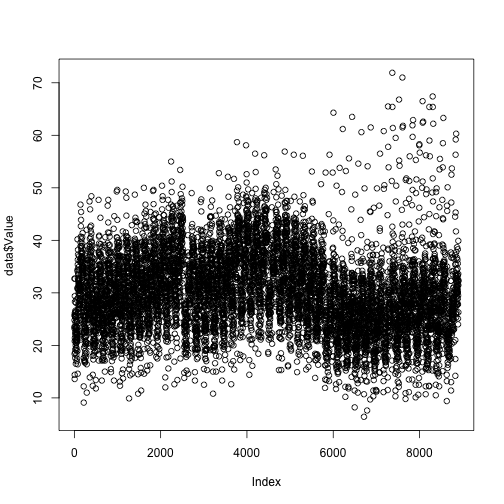
\includegraphics{SRI-Interview-App--PDF-_files/figure-latex/unnamed-chunk-2-1.pdf}

\textbf{The observation parallels the most recent article by SRI on
medium.com:}\\
\href{https://medium.com/dish/sri-research-points-to-a-tripling-of-depression-risk-in-emerging-adults-during-the-pandemic-c39819c00946}{SRI
research points to a tripling of depression risk in emerging adults
during the pandemic}\\
This observation can be useful both for people experiencing depression
and for researchers as another point of view.

\textbf{Steps:}\\
1. Datasets loading and preparation.\\
2. EDA: build time series charts.\\
3. Select null hypothesis. Define model.\\
4. Calculate the correlation coefficient, build linear regression
model.\\
5. Summary.\\
6. Conclusion.\\
7. References.

\hypertarget{datasets-loading-and-preparation}{%
\subsubsection{1. Datasets loading and
preparation}\label{datasets-loading-and-preparation}}

\textbf{Load dataset ``Indicators of Anxiety or Depression Based on
Reported Frequency of Symptoms During Last 7 Days''.}\\
\href{https://data.cdc.gov/NCHS/Indicators-of-Anxiety-or-Depression-Based-on-Repor/8pt5-q6wp}{Dataset/Variables
description} (source: data.cdc.gov)

\begin{Shaded}
\begin{Highlighting}[]
\FunctionTok{library}\NormalTok{(dplyr, }\AttributeTok{warn.conflicts =} \ConstantTok{FALSE}\NormalTok{)}
\FunctionTok{library}\NormalTok{(lubridate, }\AttributeTok{warn.conflicts =} \ConstantTok{FALSE}\NormalTok{)}
\FunctionTok{library}\NormalTok{(ggplot2)}
\FunctionTok{library}\NormalTok{(shiny)}
\FunctionTok{options}\NormalTok{(}\AttributeTok{scipen=}\DecValTok{999}\NormalTok{) }

\NormalTok{data\_survey }\OtherTok{\textless{}{-}} \FunctionTok{read.csv}\NormalTok{(}\StringTok{"https://data.cdc.gov/api/views/8pt5{-}q6wp/rows.csv?accessType=DOWNLOAD"}\NormalTok{)}
\FunctionTok{head}\NormalTok{(data\_survey)}
\end{Highlighting}
\end{Shaded}

\begin{verbatim}
##                         Indicator             Group         State      Subgroup
## 1 Symptoms of Depressive Disorder National Estimate United States United States
## 2 Symptoms of Depressive Disorder            By Age United States 18 - 29 years
## 3 Symptoms of Depressive Disorder            By Age United States 30 - 39 years
## 4 Symptoms of Depressive Disorder            By Age United States 40 - 49 years
## 5 Symptoms of Depressive Disorder            By Age United States 50 - 59 years
## 6 Symptoms of Depressive Disorder            By Age United States 60 - 69 years
##   Phase Time.Period    Time.Period.Label Time.Period.Start.Date
## 1     1           1 Apr 23 - May 5, 2020             04/23/2020
## 2     1           1 Apr 23 - May 5, 2020             04/23/2020
## 3     1           1 Apr 23 - May 5, 2020             04/23/2020
## 4     1           1 Apr 23 - May 5, 2020             04/23/2020
## 5     1           1 Apr 23 - May 5, 2020             04/23/2020
## 6     1           1 Apr 23 - May 5, 2020             04/23/2020
##   Time.Period.End.Date Value Low.CI High.CI Confidence.Interval Quartile.Range
## 1           05/05/2020  23.5   22.7    24.3         22.7 - 24.3               
## 2           05/05/2020  32.7   30.2    35.2         30.2 - 35.2               
## 3           05/05/2020  25.7   24.1    27.3         24.1 - 27.3               
## 4           05/05/2020  24.8   23.3    26.2         23.3 - 26.2               
## 5           05/05/2020  23.2   21.5    25.0         21.5 - 25.0               
## 6           05/05/2020  18.4   17.0    19.7         17.0 - 19.7
\end{verbatim}

\textbf{Filter down focus group: Var.1: ``Depression Value'' Var.2:
``Female''.}

\begin{Shaded}
\begin{Highlighting}[]
\NormalTok{data\_survey\_1 }\OtherTok{\textless{}{-}}\NormalTok{ data\_survey[}\FunctionTok{which}\NormalTok{(data\_survey}\SpecialCharTok{$}\NormalTok{Indicator }\SpecialCharTok{==} \StringTok{\textquotesingle{}Symptoms of Depressive Disorder\textquotesingle{}}
          \SpecialCharTok{\&}\NormalTok{ data\_survey}\SpecialCharTok{$}\NormalTok{Group }\SpecialCharTok{==} \StringTok{\textquotesingle{}By Sex\textquotesingle{}}
          \SpecialCharTok{\&}\NormalTok{ data\_survey}\SpecialCharTok{$}\NormalTok{Subgroup }\SpecialCharTok{==} \StringTok{\textquotesingle{}Female\textquotesingle{}}\NormalTok{),]}
\end{Highlighting}
\end{Shaded}

\textbf{Convert Date field / drop NA.}

\begin{Shaded}
\begin{Highlighting}[]
\NormalTok{data\_survey\_2 }\OtherTok{\textless{}{-}}\NormalTok{ data\_survey\_1 }\SpecialCharTok{\%\textgreater{}\%}\NormalTok{ dplyr}\SpecialCharTok{::}\FunctionTok{select}\NormalTok{(Time.Period.End.Date, Value)}
\NormalTok{data\_survey\_2}\SpecialCharTok{$}\NormalTok{Time.Period.End.Date }\OtherTok{\textless{}{-}} \FunctionTok{mdy}\NormalTok{(data\_survey\_2}\SpecialCharTok{$}\NormalTok{Time.Period.End.Date)}
\NormalTok{data\_survey\_3 }\OtherTok{\textless{}{-}}\NormalTok{ data\_survey\_2[}\FunctionTok{complete.cases}\NormalTok{(data\_survey\_2), ]}
\end{Highlighting}
\end{Shaded}

\textbf{Load dataset ``United States COVID-19 Cases and Deaths by State
over Time.}\\
\href{https://data.cdc.gov/Case-Surveillance/United-States-COVID-19-Cases-and-Deaths-by-State-o/9mfq-cb36}{Dataset/Variables
description} (source: data.cdc.gov)

\begin{Shaded}
\begin{Highlighting}[]
\NormalTok{data\_COVID19 }\OtherTok{\textless{}{-}} \FunctionTok{read.csv}\NormalTok{(}\StringTok{"https://data.cdc.gov/api/views/9mfq{-}cb36/rows.csv?accessType=DOWNLOAD"}\NormalTok{)}
\FunctionTok{head}\NormalTok{(data\_survey)}
\end{Highlighting}
\end{Shaded}

\begin{verbatim}
##                         Indicator             Group         State      Subgroup
## 1 Symptoms of Depressive Disorder National Estimate United States United States
## 2 Symptoms of Depressive Disorder            By Age United States 18 - 29 years
## 3 Symptoms of Depressive Disorder            By Age United States 30 - 39 years
## 4 Symptoms of Depressive Disorder            By Age United States 40 - 49 years
## 5 Symptoms of Depressive Disorder            By Age United States 50 - 59 years
## 6 Symptoms of Depressive Disorder            By Age United States 60 - 69 years
##   Phase Time.Period    Time.Period.Label Time.Period.Start.Date
## 1     1           1 Apr 23 - May 5, 2020             04/23/2020
## 2     1           1 Apr 23 - May 5, 2020             04/23/2020
## 3     1           1 Apr 23 - May 5, 2020             04/23/2020
## 4     1           1 Apr 23 - May 5, 2020             04/23/2020
## 5     1           1 Apr 23 - May 5, 2020             04/23/2020
## 6     1           1 Apr 23 - May 5, 2020             04/23/2020
##   Time.Period.End.Date Value Low.CI High.CI Confidence.Interval Quartile.Range
## 1           05/05/2020  23.5   22.7    24.3         22.7 - 24.3               
## 2           05/05/2020  32.7   30.2    35.2         30.2 - 35.2               
## 3           05/05/2020  25.7   24.1    27.3         24.1 - 27.3               
## 4           05/05/2020  24.8   23.3    26.2         23.3 - 26.2               
## 5           05/05/2020  23.2   21.5    25.0         21.5 - 25.0               
## 6           05/05/2020  18.4   17.0    19.7         17.0 - 19.7
\end{verbatim}

\textbf{Filter down focus group: Var.1: ``Date'' Var.2: ``Number of
cases''.}

\begin{Shaded}
\begin{Highlighting}[]
\NormalTok{data\_COVID19\_2 }\OtherTok{\textless{}{-}}\NormalTok{ data\_COVID19 }\SpecialCharTok{\%\textgreater{}\%}\NormalTok{ dplyr}\SpecialCharTok{::}\FunctionTok{select}\NormalTok{(submission\_date, new\_case)}
\NormalTok{data\_COVID19\_2}\SpecialCharTok{$}\NormalTok{submission\_date }\OtherTok{\textless{}{-}} \FunctionTok{mdy}\NormalTok{(data\_COVID19\_2}\SpecialCharTok{$}\NormalTok{submission\_date)}
\NormalTok{data\_COVID19\_2 }\OtherTok{\textless{}{-}}\NormalTok{ data\_COVID19\_2 }\SpecialCharTok{\%\textgreater{}\%} \FunctionTok{filter}\NormalTok{(new\_case }\SpecialCharTok{\textgreater{}} \DecValTok{0} \SpecialCharTok{\&}\NormalTok{ submission\_date }\SpecialCharTok{\textless{}=} \FunctionTok{as.Date}\NormalTok{(}\StringTok{\textquotesingle{}2021{-}12{-}13\textquotesingle{}}\NormalTok{))}
\end{Highlighting}
\end{Shaded}

\textbf{Grouping number of cases by day.}

\begin{Shaded}
\begin{Highlighting}[]
\NormalTok{data\_COVID19\_3 }\OtherTok{\textless{}{-}}\NormalTok{ data\_COVID19\_2 }\SpecialCharTok{\%\textgreater{}\%}
  \FunctionTok{group\_by}\NormalTok{(submission\_date) }\SpecialCharTok{\%\textgreater{}\%}
  \FunctionTok{summarize}\NormalTok{(}\AttributeTok{new\_case\_daily =} \FunctionTok{sum}\NormalTok{(new\_case, }\AttributeTok{na.rm =} \ConstantTok{TRUE}\NormalTok{))}
\end{Highlighting}
\end{Shaded}

\hypertarget{eda-build-time-series-charts.}{%
\subsubsection{2. EDA: build time series
charts.}\label{eda-build-time-series-charts.}}

\textbf{EDA: build graph to reflect number of cases daily (06/2020 -
12/2021).}

\begin{Shaded}
\begin{Highlighting}[]
\FunctionTok{ggplot}\NormalTok{(data\_COVID19\_3) }\SpecialCharTok{+}
  \FunctionTok{aes}\NormalTok{(}\AttributeTok{x =}\NormalTok{ submission\_date, }\AttributeTok{y =}\NormalTok{ new\_case\_daily, }\AttributeTok{colour =}\NormalTok{ new\_case\_daily) }\SpecialCharTok{+}
  \FunctionTok{geom\_line}\NormalTok{(}\AttributeTok{size =}\NormalTok{ 1L) }\SpecialCharTok{+}
  \FunctionTok{scale\_color\_distiller}\NormalTok{(}\AttributeTok{palette =} \StringTok{"Blues"}\NormalTok{, }\AttributeTok{direction =} \DecValTok{1}\NormalTok{) }\SpecialCharTok{+}
  \FunctionTok{labs}\NormalTok{(}\AttributeTok{title =} \StringTok{"COVID19 cases per day"}\NormalTok{,}\AttributeTok{x =} \ConstantTok{NULL}\NormalTok{, }\AttributeTok{y =} \StringTok{\textquotesingle{}COVID{-}19 Cases\textquotesingle{}}\NormalTok{) }\SpecialCharTok{+}
  \FunctionTok{ylim}\NormalTok{(}\DecValTok{0}\NormalTok{, }\DecValTok{700000}\NormalTok{) }\SpecialCharTok{+}
  \FunctionTok{scale\_x\_date}\NormalTok{(}\AttributeTok{limit=}\FunctionTok{c}\NormalTok{(}\FunctionTok{as.Date}\NormalTok{(}\StringTok{\textquotesingle{}2020{-}06{-}01\textquotesingle{}}\NormalTok{), }\FunctionTok{as.Date}\NormalTok{(}\StringTok{\textquotesingle{}2021{-}12{-}13\textquotesingle{}}\NormalTok{))) }\SpecialCharTok{+}
  \FunctionTok{theme\_classic}\NormalTok{()}
\end{Highlighting}
\end{Shaded}

\begin{verbatim}
## Warning: Removed 114 rows containing missing values (geom_path).
\end{verbatim}

\includegraphics{SRI-Interview-App--PDF-_files/figure-latex/unnamed-chunk-9-1.pdf}

\textbf{EDA: build graph to reflect Depression Value daily (05/2020 -
12-2021).}

\begin{Shaded}
\begin{Highlighting}[]
\FunctionTok{ggplot}\NormalTok{(data\_survey\_3) }\SpecialCharTok{+}
  \FunctionTok{aes}\NormalTok{(}\AttributeTok{x =}\NormalTok{ Time.Period.End.Date, }\AttributeTok{y =}\NormalTok{ Value, }\AttributeTok{colour =}\NormalTok{ Value) }\SpecialCharTok{+}
  \FunctionTok{geom\_line}\NormalTok{(}\AttributeTok{size =}\NormalTok{ 1L) }\SpecialCharTok{+}
  \FunctionTok{scale\_color\_distiller}\NormalTok{(}\AttributeTok{palette =} \StringTok{\textquotesingle{}Reds\textquotesingle{}}\NormalTok{, }\AttributeTok{direction =} \DecValTok{1}\NormalTok{) }\SpecialCharTok{+}
  \FunctionTok{labs}\NormalTok{(}\AttributeTok{title =} \StringTok{\textquotesingle{}Depression Value per day\textquotesingle{}}\NormalTok{,}\AttributeTok{x =} \ConstantTok{NULL}\NormalTok{,}\AttributeTok{y =} \StringTok{\textquotesingle{}Depression Value\textquotesingle{}}\NormalTok{) }\SpecialCharTok{+}
  \FunctionTok{theme\_classic}\NormalTok{() }\SpecialCharTok{+}
  \FunctionTok{ylim}\NormalTok{(}\DecValTok{0}\NormalTok{, }\DecValTok{40}\NormalTok{)}
\end{Highlighting}
\end{Shaded}

\includegraphics{SRI-Interview-App--PDF-_files/figure-latex/unnamed-chunk-10-1.pdf}

\hypertarget{select-null-hypothesis.-define-model.}{%
\subsubsection{3. Select null hypothesis. Define
model.}\label{select-null-hypothesis.-define-model.}}

\textbf{Null hypothesis} is female Depression appearance or increasing
doesn't have a relationship with intensity of COVID-19 pandemic.\\
To \textbf{accept} or \textbf{reject} that hypothesis linear regression
model is applied.

\hypertarget{calculate-correlation-coefficient-of-depression-value-and-covid-19-cases-per-day.}{%
\subsubsection{4. Calculate correlation coefficient of Depression Value
and COVID-19 cases per
day.}\label{calculate-correlation-coefficient-of-depression-value-and-covid-19-cases-per-day.}}

Build linear regression model.\\
\textbf{Merge datasets. Number of cases and Depression Value aggregated
by day.}

\begin{Shaded}
\begin{Highlighting}[]
\NormalTok{data\_joined }\OtherTok{\textless{}{-}} \FunctionTok{merge}\NormalTok{(}\AttributeTok{x =}\NormalTok{ data\_survey\_3, }\AttributeTok{y =}\NormalTok{ data\_COVID19\_3, }\AttributeTok{by.x=}\FunctionTok{c}\NormalTok{(}\StringTok{\textquotesingle{}Time.Period.End.Date\textquotesingle{}}\NormalTok{), }\AttributeTok{by.y=}\FunctionTok{c}\NormalTok{(}\StringTok{\textquotesingle{}submission\_date\textquotesingle{}}\NormalTok{))}
\end{Highlighting}
\end{Shaded}

\textbf{Add new column: rolling Correlation coefficient (Pearson
method).}

\begin{Shaded}
\begin{Highlighting}[]
\NormalTok{data\_joined[ , }\StringTok{\textquotesingle{}Correlation\_Coef\textquotesingle{}}\NormalTok{] }\OtherTok{\textless{}{-}} \ConstantTok{NA}
\ControlFlowTok{for}\NormalTok{ (i }\ControlFlowTok{in} \DecValTok{1}\SpecialCharTok{:}\FunctionTok{nrow}\NormalTok{(data\_joined)) \{}
\NormalTok{  data\_joined[i, }\DecValTok{4}\NormalTok{] }\OtherTok{=} \FunctionTok{as.numeric}\NormalTok{(}\FunctionTok{cor}\NormalTok{(data\_joined[}\DecValTok{1}\SpecialCharTok{:}\NormalTok{i, }\DecValTok{2}\NormalTok{], data\_joined[}\DecValTok{1}\SpecialCharTok{:}\NormalTok{i, }\DecValTok{3}\NormalTok{]))\}}
\NormalTok{data\_joined[}\DecValTok{1}\NormalTok{, }\DecValTok{4}\NormalTok{] }\OtherTok{=} \DecValTok{0}
\NormalTok{data\_joined}\SpecialCharTok{$}\NormalTok{Correlation\_Coef }\OtherTok{\textless{}{-}} \FunctionTok{round}\NormalTok{(data\_joined}\SpecialCharTok{$}\NormalTok{Correlation\_Coef, }\AttributeTok{digits =} \DecValTok{2}\NormalTok{)}
\end{Highlighting}
\end{Shaded}

\textbf{EDA: Combine graphs: Depression Value + COVID19 cases + rolling
Corr. coef.}

\begin{Shaded}
\begin{Highlighting}[]
\FunctionTok{ggplot}\NormalTok{(}\AttributeTok{data =}\NormalTok{ data\_joined) }\SpecialCharTok{+}
  \FunctionTok{geom\_line}\NormalTok{(}\FunctionTok{aes}\NormalTok{(}\AttributeTok{x =}\NormalTok{ Time.Period.End.Date, }\AttributeTok{y =}\NormalTok{ new\_case\_daily }\SpecialCharTok{/} \DecValTok{10000}\NormalTok{), }\AttributeTok{color=}\StringTok{\textquotesingle{}blue\textquotesingle{}}\NormalTok{) }\SpecialCharTok{+}
  \FunctionTok{geom\_line}\NormalTok{(}\FunctionTok{aes}\NormalTok{(}\AttributeTok{x =}\NormalTok{ Time.Period.End.Date, }\AttributeTok{y =}\NormalTok{ Value), }\AttributeTok{color=}\StringTok{\textquotesingle{}red\textquotesingle{}}\NormalTok{) }\SpecialCharTok{+}
  \FunctionTok{aes}\NormalTok{(}\AttributeTok{x =}\NormalTok{ Time.Period.End.Date, }\AttributeTok{y =}\NormalTok{ Correlation\_Coef }\SpecialCharTok{*} \DecValTok{10} \SpecialCharTok{+} \DecValTok{50}\NormalTok{, }\AttributeTok{color =}\NormalTok{ Correlation\_Coef) }\SpecialCharTok{+}
  \FunctionTok{labs}\NormalTok{(}\AttributeTok{x =} \ConstantTok{NULL}\NormalTok{, }\AttributeTok{y =} \ConstantTok{NULL}\NormalTok{, }\AttributeTok{title =} \StringTok{\textquotesingle{}COVID{-}19 cases | Depression Value | Rolling Correlation coef\textquotesingle{}}\NormalTok{) }\SpecialCharTok{+}
  \FunctionTok{geom\_point}\NormalTok{(}\AttributeTok{shape =} \StringTok{\textquotesingle{}circle\textquotesingle{}}\NormalTok{) }\SpecialCharTok{+}
  \FunctionTok{lims}\NormalTok{(}\AttributeTok{y =} \FunctionTok{c}\NormalTok{(}\DecValTok{0}\NormalTok{, }\DecValTok{100}\NormalTok{)) }\SpecialCharTok{+}
  \FunctionTok{scale\_x\_date}\NormalTok{(}\AttributeTok{limit=}\FunctionTok{c}\NormalTok{(}\FunctionTok{as.Date}\NormalTok{(}\StringTok{\textquotesingle{}2020{-}06{-}01\textquotesingle{}}\NormalTok{), }\FunctionTok{as.Date}\NormalTok{(}\StringTok{\textquotesingle{}2021{-}12{-}13\textquotesingle{}}\NormalTok{)), }\AttributeTok{date\_breaks =} \StringTok{\textquotesingle{}3 month\textquotesingle{}}\NormalTok{, }\AttributeTok{date\_labels=}\StringTok{\textquotesingle{}\%Y/\%m\textquotesingle{}}\NormalTok{) }\SpecialCharTok{+}
  \FunctionTok{theme\_classic}\NormalTok{()}
\end{Highlighting}
\end{Shaded}

\begin{verbatim}
## Warning: Removed 4 rows containing missing values (geom_path).

## Warning: Removed 4 rows containing missing values (geom_path).
\end{verbatim}

\begin{verbatim}
## Warning: Removed 4 rows containing missing values (geom_point).
\end{verbatim}

\includegraphics{SRI-Interview-App--PDF-_files/figure-latex/unnamed-chunk-13-1.pdf}
Overlaying graphs under a common scale (Y-axis) allows you to see the
relationship between variables until mid-2021. Further, the correlation
decreases.

\textbf{Build LR model.}

\begin{Shaded}
\begin{Highlighting}[]
\NormalTok{linear\_regression }\OtherTok{=} \FunctionTok{lm}\NormalTok{(Value }\SpecialCharTok{\textasciitilde{}}\NormalTok{ new\_case\_daily, }\AttributeTok{data =}\NormalTok{ data\_joined)}
\FunctionTok{summary}\NormalTok{(linear\_regression)}
\end{Highlighting}
\end{Shaded}

\begin{verbatim}
## 
## Call:
## lm(formula = Value ~ new_case_daily, data = data_joined)
## 
## Residuals:
##     Min      1Q  Median      3Q     Max 
## -6.0507 -2.6301  0.7231  2.0666  4.6061 
## 
## Coefficients:
##                    Estimate   Std. Error t value            Pr(>|t|)    
## (Intercept)    25.640996735  0.706207121  36.308 <0.0000000000000002 ***
## new_case_daily  0.000016628  0.000008143   2.042              0.0481 *  
## ---
## Signif. codes:  0 '***' 0.001 '**' 0.01 '*' 0.05 '.' 0.1 ' ' 1
## 
## Residual standard error: 2.739 on 38 degrees of freedom
## Multiple R-squared:  0.09888,    Adjusted R-squared:  0.07516 
## F-statistic:  4.17 on 1 and 38 DF,  p-value: 0.04814
\end{verbatim}

\hypertarget{summary.}{%
\subsubsection{5. Summary.}\label{summary.}}

\textbf{P-value} (0.04814) is less than 0.05 which means the
\textbf{relationship is statistically significant} and indicates strong
evidence against the null hypothesis.

\hypertarget{conslusion.}{%
\subsubsection{6. Conslusion.}\label{conslusion.}}

There is a relationship between the occurrence of female depression and
the intensity of the COVID-19 pandemic. Based on the rolling correlation
coefficient, the strongest relationship was observed in the first year
of the pandemic. Since the second half of 2021, the relationship has
been gradually decreasing. This can be interpreted as an acquired
tolerance to the pandemic.

\hypertarget{references.}{%
\subsubsection{6. References.}\label{references.}}

Datasets, support files, .PDF version of the observation are available
in the \href{https://github.com/5filipp/SRI_interview.git}{Github repo}

\end{document}
